
%------------------------------------------------
\section{Second Section}
%------------------------------------------------

\begin{frame}
\frametitle{Table}
\begin{table}
\begin{tabular}{l l l}
\toprule
\textbf{Treatments} & \textbf{Response 1} & \textbf{Response 2}\\
\midrule
Treatment 1 & 0.0003262 & 0.562 \\
Treatment 2 & 0.0015681 & 0.910 \\
Treatment 3 & 0.0009271 & 0.296 \\
\bottomrule
\end{tabular}
\caption{Table caption}
\end{table}
\end{frame}
\note[itemize]{
    \item pt 1
    \item pt 2
}

%------------------------------------------------

\begin{frame}
\frametitle{Theorem}
\begin{theorem}[Mass--energy equivalence]
$E = mc^2$
\end{theorem}
\end{frame}
\note[itemize]{
    \item pt 1
    \item pt 2
}

%------------------------------------------------


\begin{frame}
\frametitle{Imagetest}
\begin{figure}[h]
  \centering
  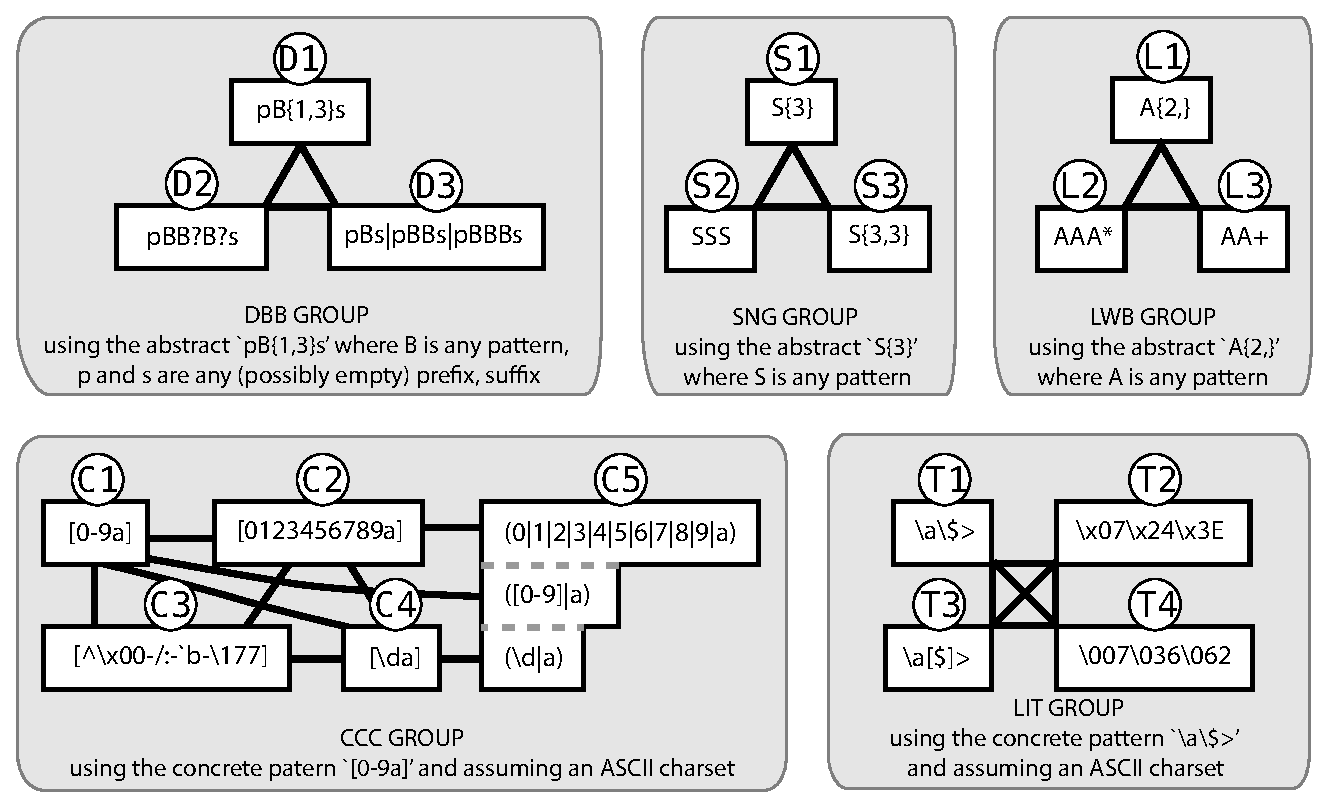
\includegraphics[scale=0.4]{nontex/illustrations/refactoringTree.eps}
  \caption{Equivalence classes with various representations of semantically equivalent representations within each class. DBB = Double-Bounded, SNG = Single Bounded, LWB = Lower Bounded, CCC = Custom Character Class and LIT = Literal}
  \label{fig:refactoringTree}
\end{figure}
\end{frame}
\note[itemize]{
    \item pt 1
    \item pt 2
}
